\documentclass[../main.tex]{subfiles}

\begin{document}
\section{Task 1 -- XGBoost}
The model was trained using mostly default parameters of the Python
\verb`xgboost` module. Despite this, it managed to achieve quite tremendous
results, as visible in table \ref{table:perf}.

\subsection{Visualizations}
\begin{figure}[H]
    \centering
    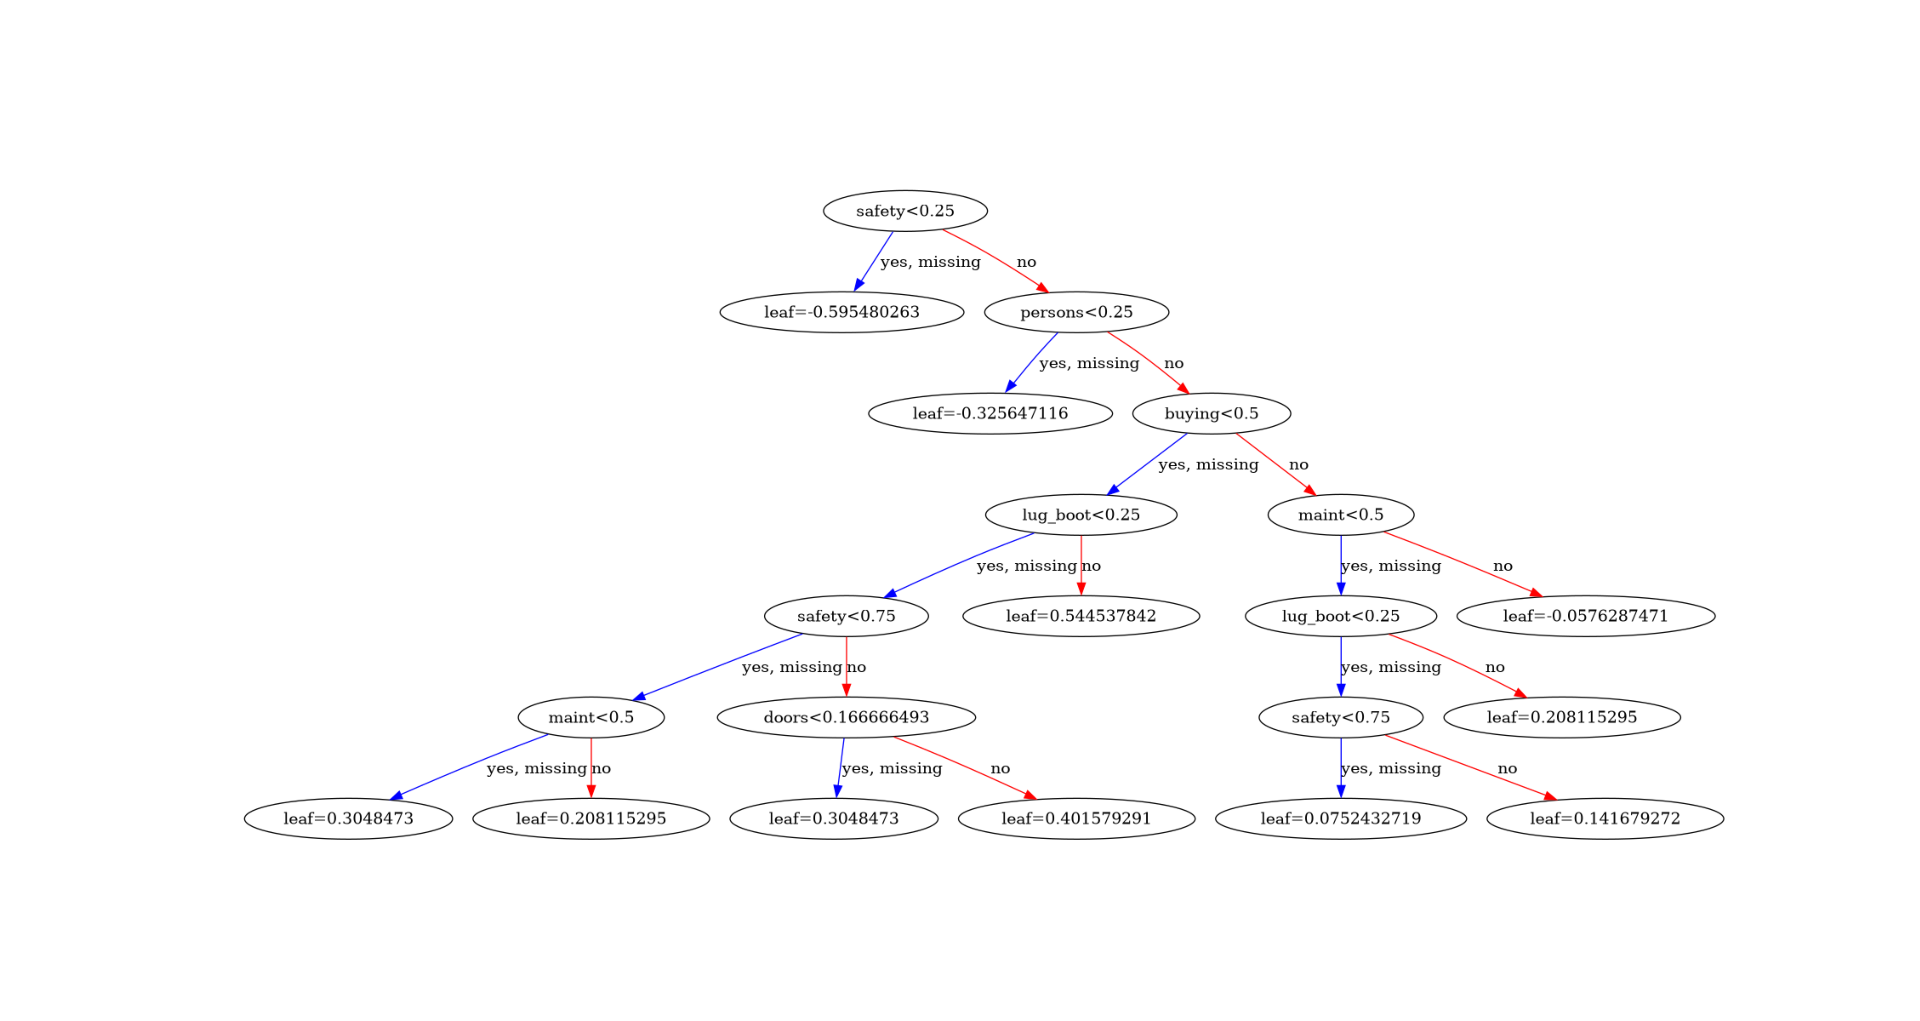
\includegraphics[width=\linewidth]{../img/xgb-tree.png}
    \caption{Last tree in the ensemble produced by XGBoost}
    \label{fig:xgb-tree}
\end{figure}
\begin{figure}[H]
    \centering
    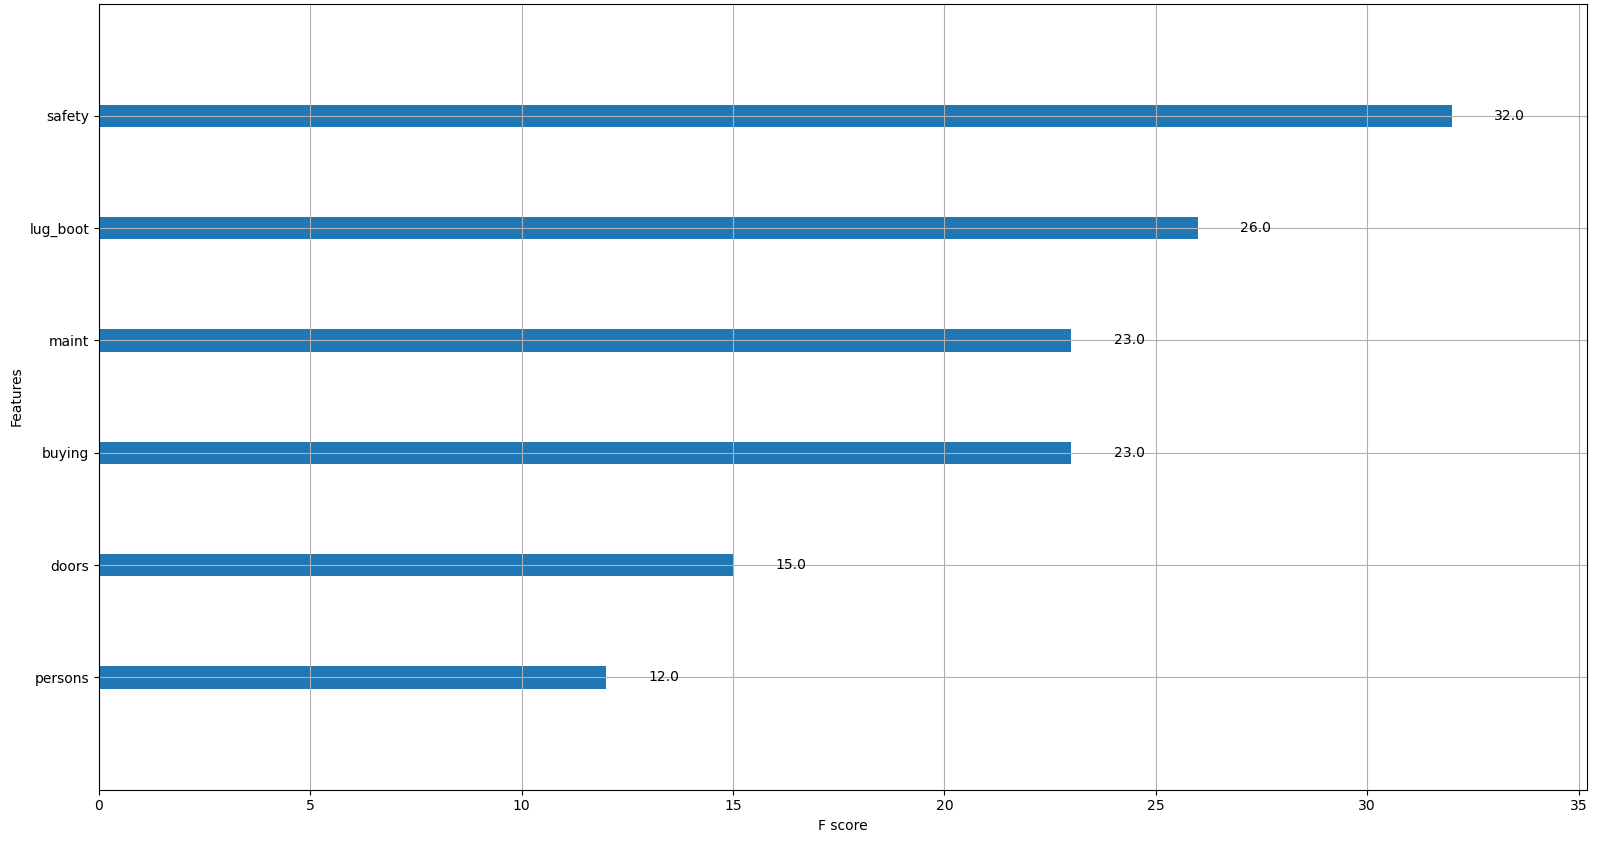
\includegraphics[width=\linewidth]{../img/xgb-feature-importance.png}
    \caption{Estimated importance of each feature}
    \label{fig:xgb-feats}
\end{figure}

\subsection{Remarks}
% TODO

\end{document}
